\chapter{Summary of Results}\label{chap:Summary}

This dissertation is based on research conducted at the University of Virginia during the period from 2014 to 2019. The bulk of the ideas have already appeared in the following two journal articles,

\begin{enumerate}
	\item `From Dirac semimetals to topological phases in three dimensions: A coupled-wire construction', Syed Raza, Alexander Sirota, and Jeffrey C. Y. Teo - Phys. Rev. X 9, 011039. \cite{RazaSirotaTeo2019}
	\item `Coupled wire models of interacting Dirac nodal superconductors' - Moon Jip Park, Syed Raza, Matthew J. Gilbert, and Jeffrey C. Y. Teo - Phys. Rev. B 98, 184514. \cite{ParkRazaGilbertTeo2018}
\end{enumerate}

Most of the passages that appear in this dissertation have been quoted verbatim from the above papers. Both of these papers were collaborative projects, my personal contributions include building the coupled-wire models for realizing Weyl and Dirac semimetals, writing symmetries that preserve the Hamiltonians, and coming up with interaction terms that satisfy the Haldane nullity conditions. For the second paper, I contributed to finding the symmetries of the coupled wire model, the symmetry-preserving relations of the Hamiltonian, and symmetry-relations for the bosonized variables and interaction terms. 

We now highlight and summarize the results presented in this dissertation. This section can also serve as a roadmap and outline for the dissertation. By mapping a Dirac (semi)metal to a model based on a three-dimensional array of wires, we show that the Dirac semimetal can acquire a many-body excitation energy gap without breaking any relevant  symmetries and leads to a three-dimensional topological order. We also construct a new interaction-enabled Dirac semimetallic state which only has a single pair of Weyl nodes and preserves time-reversal symmetry. Such a state is forbidden in a single-body setting. A general outline of the construction of both these states is given in Fig.~\ref{fig:Flowchart} and also summarized below. 

The starting point of our model is a minimal Dirac fermion model ~(\ref{DiracHam0} and Fig.~\ref{fig:Diracbands}) equipped with time-reversal and (screw) $\mathcal{C}_2$ rotation symmetries. The model is anomaly-free and so can be realized in a 3D lattice model. The first part of this article addresses a mapping between the isotropic massless Dirac fermion in the continuum limit and an anisotropic coupled wire model where the effective low-energy degrees of freedom are confined along a discrete array of 1D continuous wires. The mapping to a coupled wire model is achieved by first introducing vortices (adding mass terms) that break the symmetries microscopically (\ref{DiracHam}). These vortices are topological line defects that involve spatial winding of symmetry-breaking Dirac mass parameters. Consequently, these vortices host chiral Dirac electronic channels, each of which corresponds to a gapless quasi-1D system where electronic quasiparticles can only propagate in a single direction along the channel and are localized along the perpendiculars (\ref{lowenergy}).	

When assembled together onto a vortex lattice, the system recovers the screw $\mathcal{C}_2$ rotation symmetry as well as a set of emergent antiferromagnetic symmetries, which are combinations of the broken time-reversal and half-translations (Fig.~\ref{fig:vortexlattice}). Upon nearest-wire single-body electron backscatterings, the electronic band structure in low-energies disperses linearly and mirrors that of the continuous isotropic Dirac parent state. A symmetry-protected massless Dirac fermion (equivalently a pair of Weyl fermions with opposite chiralities) emerges and captures the low-energy long length scale electronic properties (Figs.~\ref{fig:WeylTB} and \ref{fig:Weylspectrum}). The coupled wire Dirac model and its massless energy spectrum are anomalous with respect to the \AFTR and $\mathcal{C}_2$ symmetry. The three possible resolutions of the anomaly are disussed in Sec.~\ref{sec:anomaly}. The model with an enlarged unit cell which leads to the two momentum-separated Weyl points to collapse to a single Dirac point is also discussed (Fig.~\ref{fig:DiracTB}). The corresponding Fermi arc surface states are discussed in Sec.~\ref{sec:fermiarc1} and shown in Figs.~\ref{fig:fermiarc1} and~\ref{fig:fermiarc2}.

\begin{figure}[htbp]
	\centering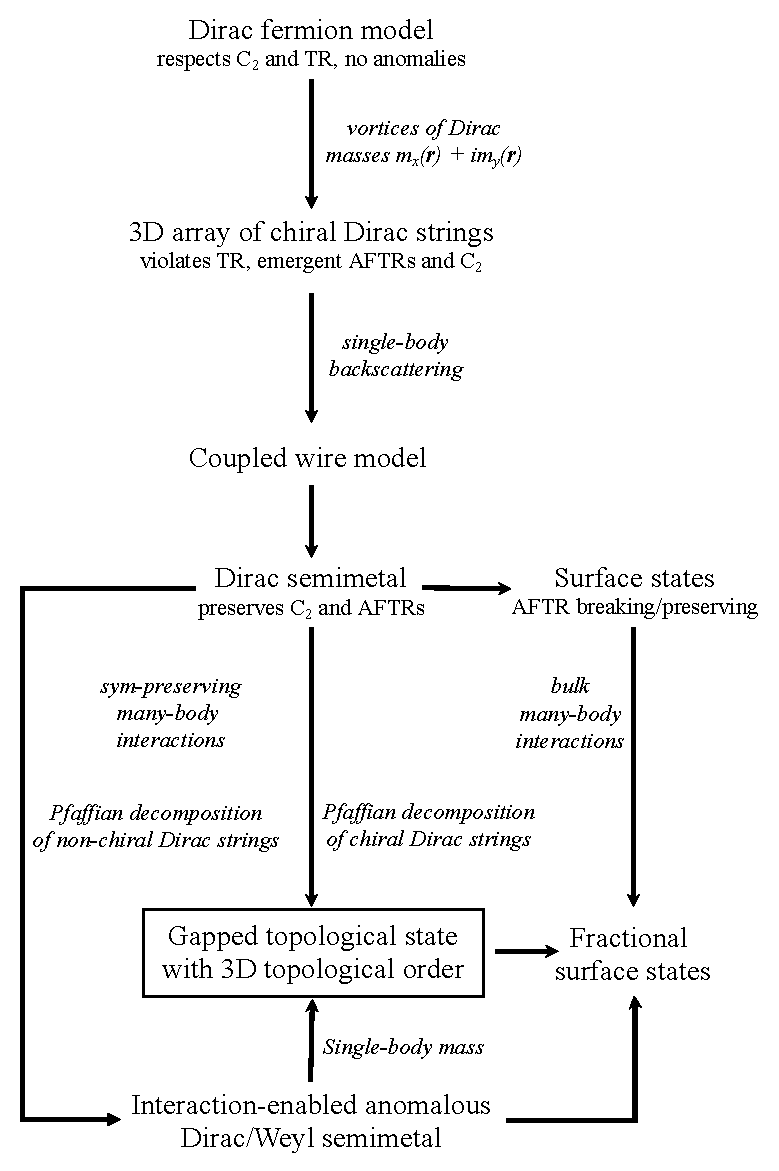
\includegraphics[width=0.8\textwidth]{Flowchart}
	\caption[Logical outline of Model 1 and Model 3.]{Logical outline of Model 1 and Model 3.  It shows the procedure of going from a Dirac fermion model to an interaction-enabled gapped state with three-dimensional topological order. Here, $\mathcal{C}_2$ is the two-fold (screw) rotation symmetry, TR is time-reversal symmetry and AFTR is the antiferromagnetic time-reversal symmetry}\label{fig:Flowchart}
\end{figure}

We then address non-trivial symmetry-preserving many-body interacting effects beyond the single-body mean-field paradigm. We begin with the anisotropic array of chiral Dirac wires that constitutes a Dirac (semi)metal protected by antiferromagnetic time-reversal (\hyperlink{AFTR}{AFTR}) and (screw) $\mathcal{C}_2$ rotation symmetries (Fig.~\ref{fig:WeylTB}). We consider an exactly-solvable model of symmetry-preserving inter-wire many-body backscattering interactions. This model is inspired by and can be regarded as a layered version of the symmetric massive interacting surface state of a topological insulator. It is based on a {\em fractionalization} scheme that divides a single chiral Dirac channel into a decoupled pair of identical chiral ``Pfaffian" channels (Fig.~\ref{fig:glueingsplitting}). Each of these fractional channels carries half of the degrees of freedom of the original Dirac wire. For instance, the fractionalization splits the electric and thermal currents exactly in half. %The bipartition is stabilized by many-body interactions and cannot be realized in any single-body mean-field description. 
It leads to the appearance of fractional quasiparticle excitations. For example, a chiral Pfaffian channel also runs along the 1D edge of the particle-hole symmetric Pfaffian fractional quantum Hall state~\cite{Son15,BarkeshliMulliganFisher15,WangSenthil16}, and supports charge $e/4$ Ising and $e/2$ semionic primary fields.

We consider an explicit combination of many-body interwire backscattering interactions that stabilize the fractionalization. Similar coupled wire constructions were applied in the literature to describe topological insulator's surface state~\cite{MrossEssinAlicea15} and $\nu=1/2$ fractional quantum Hall states~\cite{TeoKaneCouplewires,KaneSternHalperin17}. They are higher dimensional analogues of the Affleck-Kennedy-Lieb-Tasaki (AKLT) spin chain model~\cite{AKLT1,AKLT2}. The pair of chiral Pfaffian channels along each wire is backscattered in opposite directions to neighboring wires by the interaction (Fig.~\ref{fig:gappinginteraction}). As a result of this dimerization of fractional degrees of freedom, the model acquires a finite excitation energy gap and at the same time preserves the relevant symmetries.

We speculate that such a symmetry preserving-gapping by many-body interactions leads to a three-dimensional topological order supporting exotic point-like and line-like quasiparticle excitations with fractional charge and statistics. The complete characterization of the topological order will be part of a future work~\cite{SirotaRazaTeoappearsoon}. Although there have been numerous field-theoretic discussions on possible properties of topologically ordered phases in 3D, this is the first work with a microscopic model that could possibly lead to its material realization.

In the single-body regime, an (antiferromagnetic) time-reversal symmetric Weyl (semi)metal realizable on a three dimensional lattice has a minimum of four momentum-space-separated Weyl nodes. For a single pair of Weyl nodes with opposite chirality, time-reversal symmetry must be broken. However, a key result of this dissertation is the realization of a single pair of momentum-space-separated Weyl nodes in the presence of \AFTR symmetry as enabled by many-body interactions. The coupled wire construction suggests a new {\em interaction-enabled topological (semi)metal} in which these Weyl nodes can be realized (Fig.~\ref{fig:intenable}). 

The many-body interacting coupled-wire model can be turned into a gapless system, where 1) all low-energy degrees of freedom are electronic and freely described in the single-body non-interacting setting by two and only two separated Weyl nodes, 2) the high-energy gapped sector supports fractionalization. Although the model is antiferromagnetic, we conjecture that similar anomalous Weyl (semi)metal can be enabled by interaction while preserving local time-reversal.

The dissertation is organized as follows. In Sec.~\ref{sec:DiracSemimetal}, we construct a single-body coupled wire model of a Dirac/Weyl (semi)metal equipped with two emergent antiferromagnetic time-reversal (\AFTR) axes and a (screw) $\mathcal{C}_2$ rotation symmetry. In Sec.~\ref{sec:anomaly}, we establish the equivalence between the isotropic continuum limit and the anisotropic coupled wire limit by a coarse-graining mapping. We also discuss the anomalous aspects of the pair of Weyl fermions and different resolutions to the anomaly. In Sec.~\ref{sec:fermiarc1}, we describe the gapless surface states of the coupled wire model. \AFTR breaking and preserving surfaces are considered separately in Sec.~\ref{sec:fermiarcAFTRbreaking} and \ref{sec:fermiarcAFTRpreserving} respectively.

In Sec.~\ref{sec:intenable}, we move on to the effect of symmetry-preserving many-body interactions. The fractionalization of a chiral Dirac channel is explained in Sec.~\ref{sec:gluing}, where we establish the Pfaffian decomposition through bosonization techniques. The splitting of a Dirac channel is summarized in Fig.~\ref{fig:fractionalization}. In Sec.~\ref{sec:interactionmodels}, we explicitly construct an exactly-solvable interacting coupled wire model that introduces a finite excitation energy gap to the Dirac system while preserving relevant symmetries. The many-body interwire backscattering interactions are summarized in Fig.~\ref{fig:gappinginteraction}. In Sec.~\ref{sec:AFMstabilization}, we discuss a plausible stabilization mechanism of the desired interactions through an antiferromagnetic order. 

In Sec.~\ref{sec:intenable}, we discuss the other key result of the dissertation, a variation of the model that enables an anomalous topological (semi)metal. We show how a single pair of Weyl nodes in the presence of time-reversal symmetry can be realized through many-body interactions. Such a state is forbidden in the single-body setting. In Sec.~\ref{sec:fracsurface}, we elaborate on the gapless surface states of both new interacting phases discussed in sections~\ref{sec:interactionmodels} and~\ref{sec:intenable}.

We then apply similar techniques to the superconducting analogs of the Dirac semimetals known as the Dirac nodal superconductors in \ref{chap:Model3}. We repeat a similar procedure of building a wire-model and then introduce many-body interactions to gap out the system. 
We construct the many-body gapping potentials that generate a finite energy gap while preserving the underlying symmetries. In the presence of the many-body interactions, we find the emergence of the non-trivial topological orders.
We begin our discussion in Section \ref{sec:coupled} where we detail our construction the coupled wire model of a Dirac nodal superconductor in three spatial dimensions by assembling a vortex array in a microscopic superconductor within the continuum limit. In the continuum model, the massless Dirac fermions are protected by the combination of: local time-reversal symmetry, particle-hole symmetry and glide mirror symmetry. By introducing the array of superconducting pairing vortices, the low-energy electronic degrees of freedom manifest as $(1+1)$-D chiral Dirac fermions that are localized along vortex lines (also referred to as Dirac strings).  Each Dirac string is coupled via single-body tunneling with the adjacent strings, and the couplings reconstruct the Dirac nodal superconductor within the context of the coupled wire model. This anisotropic Dirac nodal superconducting model is protected by the same set of symmetries except time-reversal now becomes non-local and antiferromagnetic. This re-construction enables us to study many-body interactions in three dimensions using bosonization techniques.

With our introduction to the single body physics of the coupled wire methodology complete, in Section \ref{sec:manybody1} we introduce the many-body interactions that preserve all the underlying symmetries. The basic strategy that we follow in this work is based on the bi-partitioning the $SO(2N)$ Kac-Moody current consisting of $N$ chiral Dirac fermions along a vortex. For even $N$, the symmetric gapping interaction can be facilitated by a simple separation $SO(2N)_1\sim SO(N)_1\times SO(N)_1$ of Dirac channels. The model admits a single-body mean-field mass gap, which reflects its trivial topology under the $\mathbb{Z}_2$  classification. On the other hand, due to the presence of the aforementioned symmetries, the odd $N$ case requires a non-trivial string decomposition that involves the level-rank duality $SO(9)_1\sim SO(3)_3\times SO(3)_3$. Consequently, the gapping interactions in the case of odd $N$ lead to fractionalization and non-trivial topological order. In both situations, the gapping potentials are constructed by backscattering the divided Kac-Moody currents to opposite directions between adjacent strings. This results in a finite energy gap while preserving all the underlying symmetries of our model.

Interestingly, when $N=16$, we find a special form of the decomposition, $SO(32)\sim E_8 \times E_8$, that utilizes the $E_8$ unimodular lattice. We find that this decomposition results in the many-body interaction that has trivial topological order. 
%%